\section{Is Blockchain the Right Solution?}
\label{sec:distributed-comparison}

Blockchain technology provides a unique set of capabilities that might be better suited for a system design than competing database technologies or distributed systems.
However it does come with a relatively high overhead: replicating all past and present data and operations on the data at every node of the network in an auditable ledger.
Based on our results and experience we recommend the use of the following questions to determine if Blockchain technology would be a good fit for a specific project (see Section~\ref{sec:sharedgov} for definitions).

\begin{enumerate}
	\item Does the system require shared governance?
	\item Does the system require shared operation?
\end{enumerate}

If the answer to both questions is no, then Blockchain's consensus protocol is likely unnecessary overhead. If the answer to both questions is yes, then Blockchain technology is likely a good fit. This is due to the fact that meaningful shared governance \emph{and} operation requires miners to audit the operations of others and to be able to recover data that a malicious miner might try to delete (questions 3 and 4 below, respectively). If only shared governance or shared operation is needed, then the following two questions can be used to determine if the auditable ledger and replication, respectively, justifying the use of Blockchain technology if both are needed:

\begin{enumerate}[start=3]
	\item Is it necessary to audit the system's provenance?
	\item Is it necessary to prevent malicious data deletion?
\end{enumerate}

\subsection{Relationship to other distributed systems}
Blockchain technology fits within the broader family of distributed systems.
At the highest level, Blockchain technology is a type of decentralized database.
To help readers situate Blockchain technology within this greater ecosystem we have created a taxonomy and a flowchart based on that taxonomy (see Figure~\ref{fig:blockchainFlowchart}).

\begin{figure*}
	\centering
	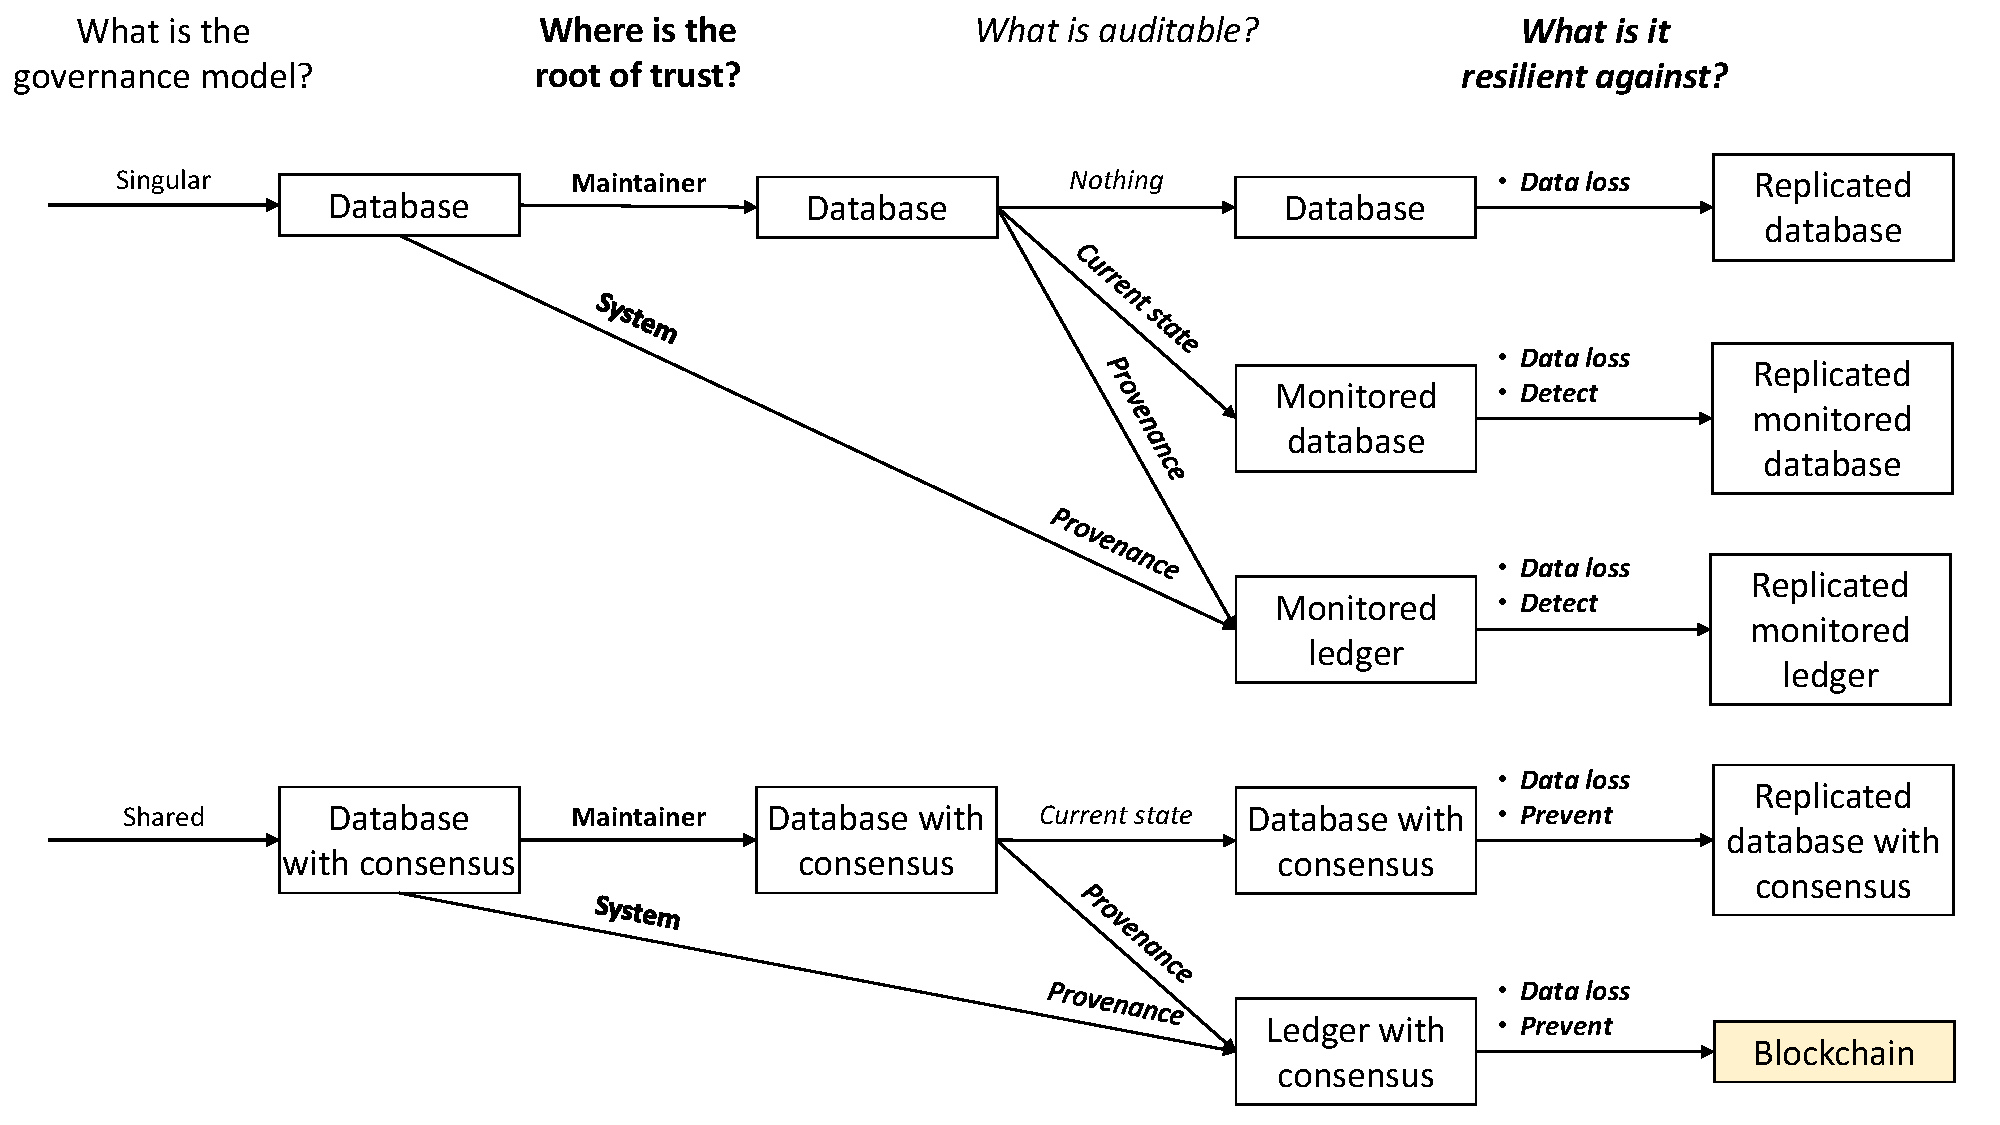
\includegraphics[width=\textwidth]{figures/BlockchainFlowchart}
	\caption{Comparing decentralized databases}
	\label{fig:blockchainFlowchart}
\end{figure*}

The first property in our taxonomy considers who has the authority to manage and update the database: \emph{what is the operation model?} In a singularly governed database (``Singular''), a single entity performs these tasks. Alternatively, the system can use a consensus protocol to allow for shared governance (``Shared'').

Next, we consider the security model by asking \emph{where is the root of trust?}
This refers to the entity or entities that must behave honestly in order for the system to be secure.
In typical database systems, trust is rooted in the maintainer (``Maintainer'')---for example, using AWS cloud storage requires that you trust Amazon.
Alternatively, trust can be rooted in the design of the system itself (``System''), though this is only possible if the system stores sufficient provenance for it to be audited to confirm that the system is functioning as intended.

The next question is \emph{what is auditable?}
In the worst case, nothing is auditable (``Nothing'').
Systems can use an authenticated data structure~\cite{tamassia2003authenticated} to ensure that their current state can be audited (``Current state'').
If the state also contains a history of the system (e.g., a ledger), then the use of an authenticated data structure allows for the provenance of the system to also be audited (``Provenance'').
In both cases, it is necessary that these databases be monitored to ensure that they never enter an invalid state, even temporarily.
In the case of shared operation, the operating entities act as monitors of the current sate during the consensus protocol.

Finally, we can classify systems by asking \emph{what is it resilient against?}
In particular, we considered with three resiliency properties---(1) is it resilient to accidental data loss (``Data loss''), (2) is it possible to detect that data has been malicious altered (``Detect''), (3) and is it possible to prevent malicious updates (``Prevent'').
Replication is a simple solution to prevent against accidental data loss, but by itself it fails to prevent malicious data loss as the malicious changes to the database will also be replicated.
In singular operation, external monitors can help detect malicious data changes, but can only do so after the data has been lost.
In shared operation, the monitors are the operators and malicious deletions and modifications will not be replicated, preventing them from effecting the overall system.